%!TEX program = lualatex

\documentclass[
	english,
	ruledheaders=section,
	%class=report,
	accentcolor=8c,
	type=intern,
	marginpar=false,
    logo=true,
	fontsize=10.5pt
	]{tudapub}

\usepackage[ngerman, main=english]{babel}
\usepackage[autostyle]{csquotes}
\usepackage{microtype}
\usepackage{seqsplit}
\usepackage{hyperref}
\usepackage{listings}
\usepackage{parskip}
\usepackage{caption}
\usepackage{cleveref}
\usepackage{biblatex}

\usepackage{tikz}
\usetikzlibrary{3d, angles, animations, arrows, arrows.meta, arrows.spaced, automata, babel, backgrounds, bending, calc, calendar, chains, circuits.ee.IEC, circuits.logic.CDH, circuits.logic.IEC, circuits.logic.US, datavisualization, datavisualization.formats.functions, datavisualization.polar, decorations, decorations.footprints, decorations.fractals, decorations.markings, decorations.pathmorphing, decorations.pathreplacing, decorations.shapes, decorations.text, er, external, fadings, fit, fixedpointarithmetic, folding, fpu, graphs, graphs.standard, intersections, lindenmayersystems, math, matrix, patterns, patterns.meta, perspective, petri, plotmarks, positioning, quotes, rdf, scopes, shadings, shadows, shadows.blur, shapes, shapes.arrows, shapes.callouts, shapes.gates.logic.IEC, shapes.gates.logic.US, shapes.geometric, shapes.misc, shapes.multipart, shapes.symbols, spy, svg.path, through, tikzmark, topaths, trees, turtle, views}

\lstdefinestyle{mystyle}{               
	captionpos=b,    
	basicstyle=\ttfamily,
	showspaces=false,                          % show spaces (with underscores)
	showstringspaces=false,            % underline spaces within strings
	showtabs=false,                            % show tabs using underscores
	frame=single,                  % adds a frame around the code
	tabsize=4,                     % default tabsize
	breaklines=true,                  % automatic line breaking
	columns=fullflexible,
	breakautoindent=false,
	framerule=1pt,
	xleftmargin=0pt,
	xrightmargin=0pt,
	breakindent=0pt,
	resetmargins=true
}
\lstset{style=mystyle}

\addbibresource{bibliography.bib} 

\begin{document}

\frontmatter

\title{Benchmarking NVSHMEM for Shuffling Operations in Distributed Database Systems}
\author{Alexander Muth, Alexander Städing, Jonas Weßner, Luis Wientgens}

\date{\today}
\maketitle

\mainmatter

\begin{abstract}
    Modern Database Management Systems (DBMSs) increasingly utilize the massively parallel architecture of Graphics Processing Units to increase performance of query operators. One building block for many query operator such as joins or aggregations is predicate-based distributed data shuffling. However one major challenge in the design for shuffling operators in GPU-accelerated distributed DBMS is the communication strategy for data exchange between nodes. The chosen strategy will impact performance and scalabilty of the shuffling operator. Specifically a common idiom in GPU-accelerated computing is to launch short GPU kernels for compute task but return to the CPU for communication. This is not optimal w.r.t the goals of performance and scalability as it introduces kernel launch overheads and forced sequentialization as well as increasing the CPU involvement. NVIDIA is actively working on GPU-initiated network communication and has recently introduced NVSHMEM, a GPU communication library that provides MPI-like communication and synchronization primitives from inside CUDA kernels. This work intends to evaluate the performance and suitability of NVSHMEM for database shuffling operators. We find that it is possible to implement shuffling over the network using NVSHMEM while achieving reasonable throughput, but also that NVSHMEM exhibits unintuitive performance characteristics and problems with the asynchronous communication interfaces that do not behave as documented. Furthermore we question the suitability of NVSHMEMs programming and memory model for the use outside of typical HPC environments.
\end{abstract}

\section{Introduction}\label{sec:intro}

As in the age of machine learning and big data the demand for storing and processing large amounts of data grows consistently, the expectations on database management systems are rising.
Since the demands of data size grow faster than the capacity of storage devices, database management systems had to adapt and move from a single-node architecture to a distributed architecture to aggregate the storage capacity of multiple computers.
However, when data is stored in a distributed fashion, processing of the data becomes more challenging, which forces database vendors to adapt their designs.
Modern database systems use sophisticated partitioning schemes and compression to reduce the size of data to be exchanged during query processing.
Furthermore, modern databases make use of specialized hardware for query processing to tackle compute intensive tasks like filtering large amounts of data based on complex expressions.
Nowadays, Graphic Processing Units (GPUs) are commonly used for query processing because their massively parallel single-instruction multiple-data (SIMD) execution model is well-suited for many database tasks which have to perform the same computations on many data elements \cite{subramanian2023}. 

A common operation to be preformed in distributed database management systems is shuffling data between nodes based on join keys to perform a join.
For this task, GPUs can be used for efficiently scanning the data and determining their destination nodes in parallel.
Once the destination of data items is known, those have to be transferred from the GPU device memory via the network interface card (NIC) to the remote node.
The conventional approach to doing this is copying the data from the GPU memory to the CPU memory and then sending the data from the CPU memory.
Since copying large amounts of data between host and device memory frequently incurs large overheads, NVIDIA developed GPUDirect \cite{gilad2011}, which allows the NIC to directly access GPU device memory.
Nevertheless, this approach is still CPU-initiated, meaning the CPU is responsible for handling the control flow of network operations. Consequently, GPU and CPU have to synchronize for each data transfer, which might cause large overheads on the database system due to repeatedly launching GPU kernels for processing parts of the data \cite{taylor2020}.
Recently, a new networking library allowing for GPU-initiated data transfers, called NVSHMEM, has been released which intends to mitigate this problem by exposing an interface very similar to the message passing interface (MPI) based on the OpenSHMEM specification for in-kernel use \cite{potluri2017} based on GPUDirect Async device initiated communication \cite{agostini2017}. This would allow for persistent kernels that can initiate network communication without the need to return control to the CPU. Therefore in this work we explore the potential and suitability of the NVSHMEM library for shuffling operations in distributed databases. We provide a series of microbenchmarks to explore the performance characteristics of NVSHMEM as well as an implementation of a GPU-driven shuffling operator.

The remainder of this work is structured as follows. In Section \ref{sec:gpuinitiated} we introduce the basic concept and terminology of CPU and GPU-initiated RDMA and explain the concept of the shared memory abstraction used in NVSHMEM. The principal concepts of distributed shuffling algorithms are explained in Section \ref{sec:shufflealgos}. In Section \ref{sec:microbench} we explore the performance characteristics of NVSHMEM communication primitives to find out which algorithmic options from Section \ref{sec:shufflealgos} should be used in the implementation in \ref{sec:impl}. Chapter \ref{sec:eval} will give an evaluation of the performance of our shuffle algorithm. Finally, we discuss our results and limitations in Section \ref{sec:discuss} and share our lessons learned and perspective on future work in Section \ref{sec:conclusion}.

% TODO: goals 


% TODO: references!


\section{GPU-inititated RDMA with NVSHMEM}\label{sec:gpuinitiated}
In the conventional approach to distributed databases, the CPU orchestrates data transfer between nodes. When using this CPU-initiated communication model, the CPU copies data from the GPU device memory to main memory.

GPUDirect \cite{gilad2011} makes it possible to avoid this copy overhead by sending data directly from the GPU.
This improved communication model using GPUDirect has a significant impact on performance, but the latency introduced from CPU initiation still leaves room for improvement: namely the removal of the CPU entirely from the communication pipeline.
This is possible with the NVSHMEM library from NVIDIA using strategies discussed in this section.

The following figures illustrate the difference in critical sections between the two approaches.

\begin{figure}[h]
    \centering
    \captionsetup{justification=centering}
    \path (0,300); %set diagram left start at 0, and has height of 300

    %Rounded Rect [id:dp602011306068072] 
    \draw   (21,106.8) .. controls (21,91.45) and (33.45,79) .. (48.8,79) -- (236.2,79) .. controls (251.55,79) and (264,91.45) .. (264,106.8) -- (264,190.2)     .. controls (264,205.55) and (251.55,218) .. (236.2,218) -- (48.8,218) .. controls (33.45,218) and (21,205.55) .. (21,190.2) -- cycle ;
    %Rounded Rect [id:dp18758960033065608] 
    \draw   (396,107.8) .. controls (396,92.45) and (408.45,80) .. (423.8,80) -- (611.2,80) .. controls (626.55,80) and (639,92.45) .. (639,107.8) --     (639,191.2) .. controls (639,206.55) and (626.55,219) .. (611.2,219) -- (423.8,219) .. controls (408.45,219) and (396,206.55) .. (396,191.2) -- cycle ;
    %Rounded Rect [id:dp6120664204960634] 
    \draw   (40,104.95) .. controls (40,97.25) and (46.25,91) .. (53.95,91) -- (95.8,91) .. controls (103.5,91) and (109.75,97.25) .. (109.75,104.95) --     (109.75,186.3) .. controls (109.75,194) and (103.5,200.25) .. (95.8,200.25) -- (53.95,200.25) .. controls (46.25,200.25) and (40,194) .. (40,186.3) --     cycle [fill={rgb:green,1;yellow,1;pink,0}];
    %Rounded Rect [id:dp21812393541423936] 
    \draw   (551,103.95) .. controls (551,96.25) and (557.25,90) .. (564.95,90) -- (606.8,90) .. controls (614.5,90) and (620.75,96.25) .. (620.75,103.95) --     (620.75,185.3) .. controls (620.75,193) and (614.5,199.25) .. (606.8,199.25) -- (564.95,199.25) .. controls (557.25,199.25) and (551,193) .. (551,185.3)     -- cycle [fill={rgb:green,1;yellow,1;pink,0}] ;
    %Rounded Rect [id:dp5570992455242908] 
    \draw   (131,101.05) .. controls (131,95.64) and (135.39,91.25) .. (140.8,91.25) -- (238.95,91.25) .. controls (244.36,91.25) and (248.75,95.64) ..     (248.75,101.05) -- (248.75,130.45) .. controls (248.75,135.86) and (244.36,140.25) .. (238.95,140.25) -- (140.8,140.25) .. controls (135.39,140.25) and     (131,135.86) .. (131,130.45) -- cycle ;
    %Rounded Rect [id:dp9865384483688472] 
    \draw   (412,101.05) .. controls (412,95.64) and (416.39,91.25) .. (421.8,91.25) -- (519.95,91.25) .. controls (525.36,91.25) and (529.75,95.64) ..     (529.75,101.05) -- (529.75,130.45) .. controls (529.75,135.86) and (525.36,140.25) .. (519.95,140.25) -- (421.8,140.25) .. controls (416.39,140.25) and     (412,135.86) .. (412,130.45) -- cycle;
    %Shape: Rectangle [id:dp5183376461620953] 
    \draw   (130,150) -- (250.75,150) -- (250.75,199.25) -- (130,199.25) -- cycle ;
    %Shape: Rectangle [id:dp2368467260325865] 
    \draw   (410,151) -- (530.75,151) -- (530.75,200.25) -- (410,200.25) -- cycle ;
    %Left Right Arrow [id:dp5286461875079793] 
    \draw  [fill={rgb, 255:red, 204; green, 76; blue, 3 }  ,fill opacity=1 ] (85.3,114.25) -- (102.8,104.25) -- (102.8,109.25) -- (137.8,109.25) --     (137.8,104.25) -- (155.3,114.25) -- (137.8,124.25) -- (137.8,119.25) -- (102.8,119.25) -- (102.8,124.25) -- cycle ;
    %Left Right Arrow [id:dp2994575111375585] 
    \draw  [fill={rgb, 255:red, 204; green, 76; blue, 3 }  ,fill opacity=1 ] (505.3,110.25) -- (522.8,100.25) -- (522.8,105.25) -- (557.8,105.25) --     (557.8,100.25) -- (575.3,110.25) -- (557.8,120.25) -- (557.8,115.25) -- (522.8,115.25) -- (522.8,120.25) -- cycle ;
    %Left Right Arrow [id:dp9904840465412947] 
    \draw  [fill={rgb, 255:red, 204; green, 76; blue, 3 }  ,fill opacity=1 ] (243.75,174.35) -- (267.57,165.25) -- (267.57,171.53) -- (392.93,171.53) --     (392.93,165.25) -- (416.75,174.35) -- (392.93,183.45) -- (392.93,177.17) -- (267.57,177.17) -- (267.57,183.45) -- cycle ;
    %Left Right Arrow [id:dp47754037113398307] 
    \draw  [fill={rgb, 255:red, 204; green, 76; blue, 3 }  ,fill opacity=1 ] (86.3,177.25) -- (103.8,167.25) -- (103.8,172.25) -- (138.8,172.25) --     (138.8,167.25) -- (156.3,177.25) -- (138.8,187.25) -- (138.8,182.25) -- (103.8,182.25) -- (103.8,187.25) -- cycle ;
    %Left Right Arrow [id:dp7512448088396187] 
    \draw  [fill={rgb, 255:red, 204; green, 76; blue, 3 }  ,fill opacity=1 ] (505.3,177.25) -- (522.8,167.25) -- (522.8,172.25) -- (557.8,172.25) --     (557.8,167.25) -- (575.3,177.25) -- (557.8,187.25) -- (557.8,182.25) -- (522.8,182.25) -- (522.8,187.25) -- cycle ;

    \draw (74.88,145.63) node   [align=left] {CPU};
    \draw (585.88,144.63) node   [align=left] {CPU};
    \draw (182.25,115.5) node   [align=left] {GPU};
    \draw (470.88,115.75) node   [align=left] {GPU};
    \draw (186.92,174.5) node   [align=left] {NIC};
    \draw (470.38,175.63) node   [align=left] {NIC};
    \caption{Communication with CPU in critical path}
    \label{fig:cpu_in_crit}
\end{figure}

In Figure \ref{fig:cpu_in_crit}, the CPU is included in the critical communication path, incurring a latency penalty.
The following Figure \ref{fig:cpu_out_crit} shows the critical communication path in the GPU initiated approach, which no longer includes the CPU.

\begin{figure}[h]
    \centering
    \captionsetup{justification=centering}
    \path (0,300); %set diagram left start at 0, and has height of 300

    %Rounded Rect [id:dp602011306068072] 
    \draw   (21,106.8) .. controls (21,91.45) and (33.45,79) .. (48.8,79) -- (236.2,79) .. controls (251.55,79) and (264,91.45) .. (264,106.8) -- (264,190.2)     .. controls (264,205.55) and (251.55,218) .. (236.2,218) -- (48.8,218) .. controls (33.45,218) and (21,205.55) .. (21,190.2) -- cycle ;
    %Rounded Rect [id:dp18758960033065608] 
    \draw   (396,107.8) .. controls (396,92.45) and (408.45,80) .. (423.8,80) -- (611.2,80) .. controls (626.55,80) and (639,92.45) .. (639,107.8) --     (639,191.2) .. controls (639,206.55) and (626.55,219) .. (611.2,219) -- (423.8,219) .. controls (408.45,219) and (396,206.55) .. (396,191.2) -- cycle ;
    %Rounded Rect [id:dp6120664204960634] 
    \draw   (40,104.95) .. controls (40,97.25) and (46.25,91) .. (53.95,91) -- (95.8,91) .. controls (103.5,91) and (109.75,97.25) .. (109.75,104.95) --     (109.75,186.3) .. controls (109.75,194) and (103.5,200.25) .. (95.8,200.25) -- (53.95,200.25) .. controls (46.25,200.25) and (40,194) .. (40,186.3) --     cycle [fill=black!40]; 
    %Rounded Rect [id:dp21812393541423936] 
    \draw   (551,103.95) .. controls (551,96.25) and (557.25,90) .. (564.95,90) -- (606.8,90) .. controls (614.5,90) and (620.75,96.25) .. (620.75,103.95) --     (620.75,185.3) .. controls (620.75,193) and (614.5,199.25) .. (606.8,199.25) -- (564.95,199.25) .. controls (557.25,199.25) and (551,193) .. (551,185.3)     -- cycle [fill=black!40];
    %Rounded Rect [id:dp5570992455242908] 
    \draw   (131,101.05) .. controls (131,95.64) and (135.39,91.25) .. (140.8,91.25) -- (238.95,91.25) .. controls (244.36,91.25) and (248.75,95.64) ..     (248.75,101.05) -- (248.75,130.45) .. controls (248.75,135.86) and (244.36,140.25) .. (238.95,140.25) -- (140.8,140.25) .. controls (135.39,140.25) and     (131,135.86) .. (131,130.45) -- cycle ;
    %Rounded Rect [id:dp9865384483688472] 
    \draw   (412,101.05) .. controls (412,95.64) and (416.39,91.25) .. (421.8,91.25) -- (519.95,91.25) .. controls (525.36,91.25) and (529.75,95.64) ..     (529.75,101.05) -- (529.75,130.45) .. controls (529.75,135.86) and (525.36,140.25) .. (519.95,140.25) -- (421.8,140.25) .. controls (416.39,140.25) and     (412,135.86) .. (412,130.45) -- cycle ;
    %Shape: Rectangle [id:dp5183376461620953] 
    \draw   (130,150) -- (250.75,150) -- (250.75,199.25) -- (130,199.25) -- cycle ;
    %Shape: Rectangle [id:dp2368467260325865] 
    \draw   (410,151) -- (530.75,151) -- (530.75,200.25) -- (410,200.25) -- cycle ;
    %Left Right Arrow [id:dp9904840465412947] 
    \draw  [fill={rgb, 255:red, 204; green, 76; blue, 3 }  ,fill opacity=1 ] (243.75,174.35) -- (267.57,165.25) -- (267.57,171.53) -- (392.93,171.53) --     (392.93,165.25) -- (416.75,174.35) -- (392.93,183.45) -- (392.93,177.17) -- (267.57,177.17) -- (267.57,183.45) -- cycle ;
    %Left Right Arrow [id:dp47754037113398307] 
    \draw  [fill={rgb, 255:red, 204; green, 76; blue, 3 }  ,fill opacity=1 ] (191.03,129.25) -- (202.75,137.25) -- (196.89,137.25) -- (196.89,153.25) --     (202.75,153.25) -- (191.03,161.25) -- (179.3,153.25) -- (185.16,153.25) -- (185.16,137.25) -- (179.3,137.25) -- cycle ;
    %Left Right Arrow [id:dp2871368640426972] 
    \draw  [fill={rgb, 255:red, 204; green, 76; blue, 3 }  ,fill opacity=1 ] (472.03,129.25) -- (483.75,137.25) -- (477.89,137.25) -- (477.89,153.25) --     (483.75,153.25) -- (472.03,161.25) -- (460.3,153.25) -- (466.16,153.25) -- (466.16,137.25) -- (460.3,137.25) -- cycle ;
    
    % Text Node
    \draw (74.88,145.63) node   [align=left] {CPU};
    % Text Node
    \draw (585.88,144.63) node   [align=left] {CPU};
    % Text Node
    \draw (182.25,115.5) node   [align=left] {GPU};
    % Text Node
    \draw (470.88,115.75) node   [align=left] {GPU};
    % Text Node
    \draw (186.92,174.5) node   [align=left] {NIC};
    % Text Node
    \draw (470.38,175.63) node   [align=left] {NIC};
    
    
    \caption{Communication with CPU out of critical path}
    \label{fig:cpu_out_crit}
\end{figure}

This paper explores this idea and its challenges using the NVSHMEM library for GPU-to-GPU communication, bypassing the latency introduced by the CPU.
Specifically, it analyzes the performance characteristics of NVSHMEM, and whether it provides a significant benefit for database workloads.

While the latency may be significantly improved with this approach, it is possible that additional complexity or issues in other metrics such as throughput make this approach unrealistic.

\clearpage

\subsection{Kernel Launch Overhead}

A common GPU programming model involves launching compute-heavy kernels on the device (GPU) and returning control to the host (CPU) before the next kernel launch.
The following Figure \ref{fig:kernel_launch_overhead} quantifies the impact of these kernel launches to assess whether this is an area of potential optimization.

\begin{figure}[h]
    \centering
    \captionsetup{justification=centering}
    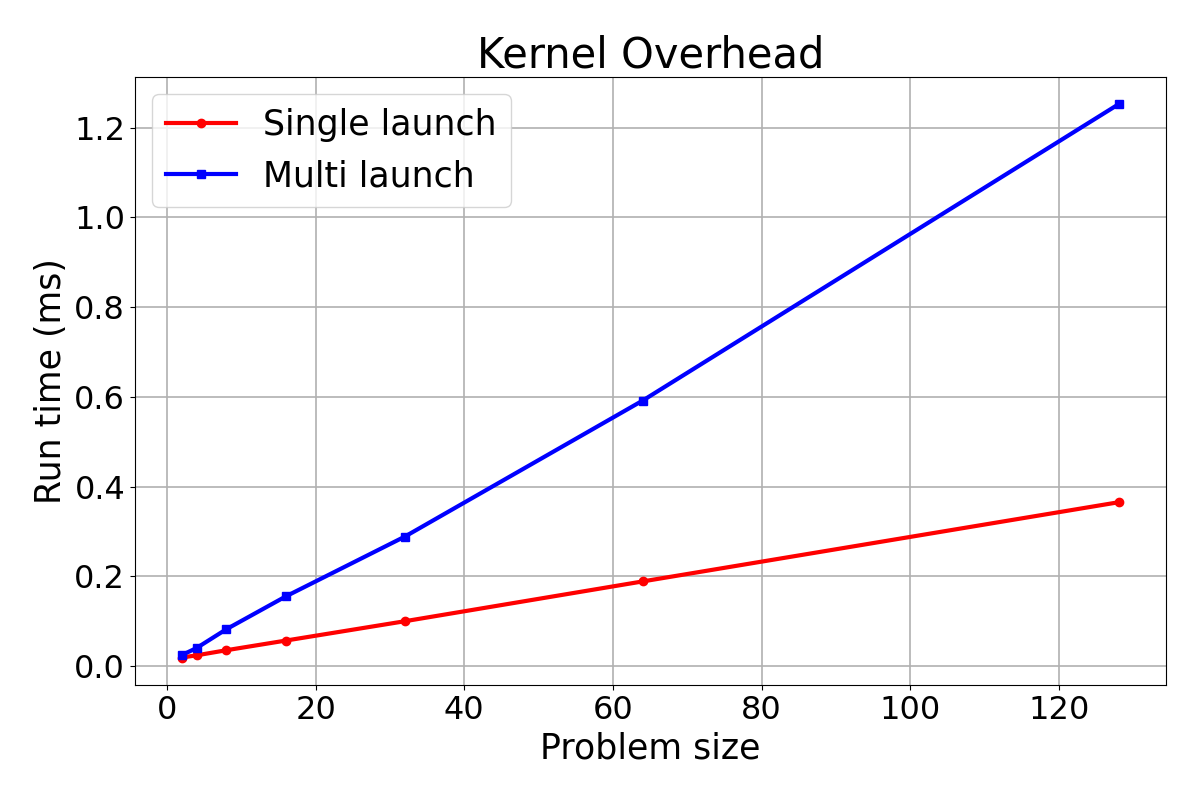
\includegraphics[width=0.4\textwidth]{img/overhead.png}
    \caption{Kernel launch overhead}
    \label{fig:kernel_launch_overhead}
\end{figure}

In this experiment, a progressively increasing problem size is tested with different kernel granularities.
The \enquote{Single launch} configuration uses a larger kernel, which is only be launched once.
On the other hand, the \enquote{Multi launch} configuration splits the work instead into smaller kernels which are launched separately.
Even though the same amount of work is completed by each configuration for a given problem size, there is a measurable increase in the kernel overhead - the time it takes to launch a kernel - for multiple kernel launches.

This serves as an important motivation to reduce the number of kernel launches in latency sensitive applications such as databases.
The problem with reducing the number of kernel launches in traditional CPU-initiated communication is that the CPU's control of the communication requires kernels to be much more fine-grained.

However, with the NVSHMEM programming model, it is possible to have much longer running kernels working more independently from the CPU, which would significantly reduce overhead induced from kernel launches.

\subsection{Programming Model}

NVSHMEM employs a programming model inspired by HPC-style computing, with the focus on cluster-wide symmetric memory exchanges.
The following Figure \ref{fig:nvshmem_sym_mem} illustrates the idea behind this symmetric memory model.

\begin{figure}[h]
    \centering
    \captionsetup{justification=centering}
    \begin{tikzpicture}[x=1pt,y=0.9pt,yscale=-0.55,xscale=0.65]
    %Rounded Rect [id:dp5682014849782169] 
    \draw   (100,34.25) .. controls (100,26.52) and (106.27,20.25) .. (114,20.25) -- (156,20.25) .. controls (163.73,20.25) and (170,26.52) .. (170,34.25) -- (170,255.25) .. controls (170,262.98) and (163.73,269.25) .. (156,269.25) -- (114,269.25) .. controls (106.27,269.25) and (100,262.98) .. (100,255.25) -- cycle ;
    %Rounded Rect [id:dp5262477048147362] 
    \draw   (191,34.25) .. controls (191,26.52) and (197.27,20.25) .. (205,20.25) -- (247,20.25) .. controls (254.73,20.25) and (261,26.52) .. (261,34.25) -- (261,255.25) .. controls (261,262.98) and (254.73,269.25) .. (247,269.25) -- (205,269.25) .. controls (197.27,269.25) and (191,262.98) .. (191,255.25) -- cycle ;
    %Rounded Rect [id:dp7573581856079369] 
    \draw   (369,35.25) .. controls (369,27.52) and (375.27,21.25) .. (383,21.25) -- (425,21.25) .. controls (432.73,21.25) and (439,27.52) .. (439,35.25) -- (439,256.25) .. controls (439,263.98) and (432.73,270.25) .. (425,270.25) -- (383,270.25) .. controls (375.27,270.25) and (369,263.98) .. (369,256.25) -- cycle ;
    %Shape: Rectangle [id:dp7570532028079713] 
    \draw  [fill={rgb, 255:red, 208; green, 2; blue, 27 }  ,fill opacity=1 ] (109.42,70.25) -- (161.42,70.25) -- (161.42,109.25) -- (109.42,109.25) -- cycle ;
    %Shape: Rectangle [id:dp19421520470566733] 
    \draw  [fill={rgb, 255:red, 208; green, 2; blue, 27 }  ,fill opacity=1 ] (199.42,71.25) -- (251.42,71.25) -- (251.42,110.25) -- (199.42,110.25) -- cycle ;
    %Shape: Rectangle [id:dp32300543498141965] 
    \draw  [fill={rgb, 255:red, 208; green, 2; blue, 27 }  ,fill opacity=1 ] (379.42,70.25) -- (431.42,70.25) -- (431.42,109.25) -- (379.42,109.25) -- cycle ;
    %Rounded Rect [id:dp6580910781722736] 
    \draw  [fill={rgb, 255:red, 126; green, 211; blue, 33 }  ,fill opacity=1 ] (111.42,141.05) .. controls (111.42,135.64) and (115.8,131.25) .. (121.22,131.25) -- (150.62,131.25) .. controls (156.03,131.25) and (160.42,135.64) .. (160.42,141.05) -- (160.42,190.45) .. controls (160.42,195.86) and (156.03,200.25) .. (150.62,200.25) -- (121.22,200.25) .. controls (115.8,200.25) and (111.42,195.86) .. (111.42,190.45) -- cycle ;
    %Rounded Rect [id:dp26363692092381197] 
    \draw  [fill={rgb, 255:red, 126; green, 211; blue, 33 }  ,fill opacity=1 ] (201.42,141.05) .. controls (201.42,135.64) and (205.8,131.25) .. (211.22,131.25) -- (240.62,131.25) .. controls (246.03,131.25) and (250.42,135.64) .. (250.42,141.05) -- (250.42,190.45) .. controls (250.42,195.86) and (246.03,200.25) .. (240.62,200.25) -- (211.22,200.25) .. controls (205.8,200.25) and (201.42,195.86) .. (201.42,190.45) -- cycle ;
    %Rounded Rect [id:dp18887280028716125] 
    \draw  [fill={rgb, 255:red, 126; green, 211; blue, 33 }  ,fill opacity=1 ] (380.42,140.05) .. controls (380.42,134.64) and (384.8,130.25) .. (390.22,130.25) -- (419.62,130.25) .. controls (425.03,130.25) and (429.42,134.64) .. (429.42,140.05) -- (429.42,189.45) .. controls (429.42,194.86) and (425.03,199.25) .. (419.62,199.25) -- (390.22,199.25) .. controls (384.8,199.25) and (380.42,194.86) .. (380.42,189.45) -- cycle ;
    %Rounded Rect [id:dp5265848887584798] 
    \draw  [color={rgb, 255:red, 0; green, 0; blue, 0 }  ,draw opacity=1 ][dash pattern={on 0.84pt off 2.51pt}] (41.42,64.65) .. controls (41.42,34.05) and (66.22,9.25) .. (96.82,9.25) -- (445.02,9.25) .. controls (475.61,9.25) and (500.42,34.05) .. (500.42,64.65) -- (500.42,230.85) .. controls (500.42,261.45) and (475.61,286.25) .. (445.02,286.25) -- (96.82,286.25) .. controls (66.22,286.25) and (41.42,261.45) .. (41.42,230.85) -- cycle ;
    %Shape: Rectangle [id:dp9039242900086101] 
    \draw  [color={rgb, 255:red, 245; green, 166; blue, 35 }  ,draw opacity=1 ][dash pattern={on 5.63pt off 4.5pt}][line width=1.5]  (106,121) -- (433.42,121) -- (433.42,210.25) -- (106,210.25) -- cycle ;
    
    % Text Node
    \draw (135.26,34.5) node   [align=left] {PE 0};
    % Text Node
    \draw (225.26,34.5) node   [align=left] {PE 1};
    % Text Node
    \draw (405.26,34.5) node   [align=left] {PE 2};
    % Text Node
    \draw (510,272) node [anchor=north west][inner sep=0.8pt]  [rotate=-270] [align=left] {NVSHMEM\_TEAM\_WORLD};
    % Text Node
    \draw (280,145) node [anchor=north west][inner sep=0.75pt]   [align=center] {Symmetric \\ Memory};
\end{tikzpicture}

    \caption{NVSHMEM symmetric memory model}
    \label{fig:nvshmem_sym_mem}
\end{figure}

In this model, a PE (Processing Element) represents a group of operating system processes, which may be executed on one or more nodes in a GPU cluster\cite{NVSHMEM2023}.
However, while it is possible to launch multiple PEs on a single GPU, this is not a recommended configuration in a production deployment, so this paper will focus on configurations with one PE per GPU and one GPU per node.

In this paper, we use NVSHMEM primitives for collective communication such as \textit{fcollect} to exchange local portions of a symmetrically allocated block with all the other PEs in the cluster.
Additionally, calls such as \textit{put\_nbi} are used for direct PE-to-PE communication.

Leveraging NVSHMEM allows us to reduce CPU involvement in data exchanges for benefits such as reduced communication latency.
However, this comes at the cost of a more complex programming model.
Compared to traditional distributed database approaches, using NVSHMEM for CPU independent communication is significantly more complex.

% - explain the difference between CPU- and GPU-initiated communicatoin
% - Explain the potential advantage of GPU-initiated communication: less kernel launch overhead, less CPU utilization, easier balance between compute and networking w/ async calls

\section{Distributed Shuffle Algorithms}\label{sec:shufflealgos}

In this chapter, we explain different algorithms relevant for shuffling in distributed database management systems of which we utilize some later in our implementation in Section \ref{sec:impl}.

The distributed shuffle is an important building block for many distributed data base algorithms such as joins and aggregations.
For a join, tuples with the same join key must be present on the same node.
Ideally, no data movement is necessary when using hash-partitioning on the join key: tuples are assigned to nodes based on the hash of their join key at the time of inserting them into the database.
However, this is not always possible because queries can use arbitrary columns as join keys but only one column can be chosen for the partitioning key.
Consequently, distributed databases have to use a shuffling algorithm to move tuples with the same key to the same node before joining those tuples.
In the following, we will step-by-step explore different algorithms for distributed shuffling

\subsection{Basic Single-threaded Scan with Two-sided communication}

To begin simple, we start with a single-threaded scan algorithm with send-receive communication.
In this algorithm, each process scans the data and performs two operations for each tuple one after another:
(1) determine its destination by calculating a hash on the shuffle key and
(2) send the tuple to the destination node.
While doing that, each process runs a receiver thread that waits for incoming messages from other nodes and stores them in a local array.
This algorithm suffers from multiple issues:
(1) the receiver uses compute resources for receiving data,
(2) the scan is single-threaded and therefore rather slow,
(3) depending on the networking primitives used, tuple-wise sending may be slow because it causes much control flow and metadata overhead,
and (4) scanning the data and sending data happen sequentially alternating, making the sending thread wait for the send operations to finish before continuing with the next tuple, thereby leaving the compute and network resources idle in the respective intervals.

\subsection{One-sided Communication}
\label{sec:shuffle:single-thread-one-sided}

Let us try to mitigate the first issue the previous algorithm and use one-sided communication between the nodes, meaning the sender stores the data directly at a specific place at the receiver (can implemented using RDMA).
In order to do that, the sender needs to know the correct storage location on the receiver.
Since each node may receive data from multiple other nodes, the send operation must be coordinated.
One approach is to use one receive buffer per node and synchronize the remote accesses of the senders, such that each sender is atomically incrementing the current offset into the array, thereby preventing any data races.
The downside of this approach is that distributed atomic operations are very costly to implement.
Another approach is to split the receive buffer into distinct parts for each peer per node.
Then each process can write into its assigned receive buffer at the remote nodes without having to synchronize with the other processes because they write to different locations in the same buffer.
In order to use this technique, each node must know where its part in the receiver's buffer begins.
To compute this information, each process must determine the data size it will send to each other node before actually sending it.
For this purpose, each process has to scan the data once and compute a histogram of how many tuples it has in its local data partition for each destination node.
Afterwards, each node $i$ must compute its own write offset $o_{i,j}$ into the buffer of each receiver $j$ as follows:
$$
o_{i,j} = \sum_{i=0}^{i-1}d_{i,j}
$$
where $d_{i,j}$ denotes the data size that node $i$ will send to node $j$.
Consequently, each node $i$ has to send the information $n_i$ to each other node $k$ with $k > i$.

\subsection{Multi-threaded Scanning}

In this implementation we parallelize the scanning of the data.
For this purpose, each thread is assigned a subset of the local data.
For this, we assume that the data size is divisible by the number of threads.
If this assumption does not hold, the implementation can leave some threads idle in the last iteration.
There are two variants of this algorithm.
The first one uses node-local synchronization for ensuring data-race free sending to remote nodes.
The other uses thread-level histograms and write offsets to achieve synchronization-free writing.
While the first variant can suffer from congestion in the synchronization primitives, the second variant has a higher computational overhead and meta data overhead.
Let us look at both variants in more detail and start with the node-level synchronizing one:

In the histogram creation phase all threads on one node build one histogram.
A possible algorithm for that is composing the histogram of $n$ atomic counters.
Then each thread can increment the respective counter as they scan over their subset of the local data.
Another possible algorithm for the histogram creation is to create thread-local histograms first and then merge them afterwards.
While the first algorithm has a smaller storage complexity, the second one suffers less from synchronization overhead.
After the histogram creation phase, the nodes exchange their histograms and build the node-level write offsets as before.
Then each node can write synchronization-free into the respective locations at the remote nodes.
But because each node has multiple threads sending at the same time, there must be proper intra-node synchronization.
For this purpose, $n$ atomic write offsets \textendash{} one for each destination \textendash{} are created and incremented by the threads as they scan through their portion of the data, ensuring data race freedom.
Note here that each thread is assigned a portion of the local tuples of known size, but the data size transferred from a particular thread to a particular node is unknown due to the key distribution.

Now we will have a look at the second variant of the multi-threaded scan algorithm.
In this algorithm we use thread-level histograms and offsets to allow for synchronization-free writing to remote nodes' storage.
In the histogram creation phase each thread builds a histogram of how many tuples it will send to each destination node.
Afterwards the thread-level histogram have to be merged into a node-level histogram by computing the component-wise sum of all histogram values across the threads.
Then each node shares the relevant parts of its node-level histogram and computes the node-level write offsets as explained in Section \ref{sec:shuffle:single-thread-one-sided}.
Furthermore, each node now also needs to compute thread-level write offsets for each destination that map distinct parts of the remote write location of one node to the individual threads on the sending node.
Creating these offsets can be achieved via a sweep-up and sweep-down algorithm. % TODO: reference, this was shown in ADMS
Once the thread-level offsets have been computed, each thread can write freely into its assigned remote location without the need of any inter- or intra-node synchronization.

\subsection{Send Buffers}
\label{sec:shuffle:send-buffers}

As touched upon earlier, the tuple-wise sending as explained in the previous algorithm versions might not be efficient depending on the communication primitives used.
There are mainly two factors that cause a detrimental effect on the sending performance when using tuple-wise sending: the control flow overhead and the metadata overhead.
The control flow overhead is caused by calling the networking primitive interface, which costs few or many cycles depending on the implementation of the used primitive.
The metadata overhead might be caused by the ratio of metadata to payload in the messages being sent to the NIC.
If the communication primitive maps one send call to one message to the NIC, tuple-wise sending causes a high metadata overhead.
In this case it might be a good idea for the shuffle implementation to assemble tuples to be send in buffers and send them out once they are full, thereby reducing the frequency and the total number of interface invocations and thereby reducing the metadata overhead. 
If, however, the networking library used is already implementing such a buffering and batch-wise sending mechanism internally, implementing buffering in the shuffle algorithm might conversely have a negative impact on performance.
In explanation, the implementation would spend cycles on assembling data in buffers just to have to buffers then be copied into a second set of buffers allocated within the networking library, thereby causing additional control flow and copying overhead.
In this subsection, we extend the algorithm from the previous subsection by implementing buffering, assuming that there is no internal buffering implemented in the networking library used.
Since there are many options to implement buffering, we show multiple alternatives.
One specific buffering strategy can be assembled by choosing from the alternatives given and putting them together in one algorithm.

The first thing to think about when implementing buffering for the shuffle algorithm is how many buffers to use.
Usually, for one invocation of the networking library's primitives, it is expected to specify exactly one destination address.
For this reason, the implementation needs at least $n$ send buffers per node for a distributed systems with $n$ nodes, one send buffer for the data going to each respective node (tuples to be kept local are modelled as sending to oneself).
The idea is to fill the buffers up using parallelized scanning and then calling the networking primitives once per buffer as soon as they are full.
When inserting into the buffers using multiple threads, we must take care of preventing data races (race conditions are usually accepted here since the order of inserts does not matter)
Depending on the hardware (e.g. NVIDIA GPU) and software (e.g CUDA, NVSHMEM) one might consider using a multiple of $n$ for the number of send buffers, since it might impact the performance of the synchronization or the sending.
For example, CUDA atomics are usually more efficient if used inside of blocks, so it might be an option to use one send buffer per block.
Also, depending implementation of the underlying networking interface used, using more blocks for sending might or might not influence the sending performance.
For simplicity, we assume exactly $n$ send buffers for the remainder of this section.
Later in our implementation in Section \ref{sec:impl} we consider the other options based on the results of our benchmarks from Section \ref{sec:microbench}.

The second issue to be considered is the synchronization when inserting into the buffers.
We give three options for this purpose:
(1) atomic insertion,
(2) local-computation and merging
(3) sync-free insertion with thread-level offsets.
For the atomic insertion strategy, the algorithm needs to allocate $n$ atomic pointer variables, one for each send buffer.
The variables store the offset to the next free position in the send buffer i.e. the position where the next tuple should be inserted.
Whenever a thread has scanned a tuple and determined its send destination to be node $i$, it will \textit{first} atomically increment the offset for send buffer $i$ and save the value of the counter before updating it.
Then it can safely insert the tuple into the location according to the offset before the update.
The order is important because the threads need to first acquire their exclusive location by updating the counter before they can safely write into the buffer.
While this synchronization approach has very low space complexity, it might suffer from congestion in the atomic operations.
The second option for synchronization, namely local-computation and merging, is implemented as follows.
Each thread allocates $n$ private buffers where it can insert the buffers without synchronizing with other threads.
Once the buffers are full, the threads merge their buffers into global buffers for sending.
Since the order of the tuples in the send buffers can be arbitrary, the merging has low computational overhead.
However, this approach requires additional copy operations (first copy into private buffers,  then copy into global buffers) and suffers from very high space complexity, which is especially on GPUs with limited RAM and issue.
The third approach using thread-level offsets is a little bit more sophisticated.
For this approach, the shuffle algorithm needs to calculate offsets analogous to explained in Section \ref{sec:shuffle:single-thread-one-sided} but with a finer granularity.
When scanning the data in the histogram creation phase, there will be created thread-level, batch-level histograms which store the information about how many tuples each thread has to send for each destination within each batch of the scanned data.
It is not sufficient to build thread-level histograms for the entire data because the data distribution is arbitrary and therefore it is necessary to know the distribution for each send batch in order to compute offsets into the send buffers per batch.
The information of the histograms is then used analogously to explained in Section \ref{sec:shuffle:single-thread-one-sided} to compute thread-level offsets per batch that denote the starting point for writing into the send buffer of the specific batch for a specific thread.
The advantage of this approach is that inserting into the send buffers is fully synchronization-free, which comes with the cost of higher algorithmic complexity, more computational overhead in the histogram creation phase and space complexity for storing the thread-level, block-level histograms and offsets

The presented alternatives to implementing the buffering, and the question on whether or not to use buffering, depend largely on the used hardware, software and the various parameters such as buffer size, number of buffers and number of threads and data size.

\subsection{Double Buffering}
\label{sec:shuffle:double-buffering}

In this subsection we address the issue of idle times during computing and networking phases.
When using blocking networking primitives, the computing resources idle while when a the set of send buffers is being sent out.
Conversely, when using an asynchronous networking interface, the calls to the send primitives return immediately and the networking is done in the background.
In order to leverage the power of non-blocking networking primitives to reduce idle times in our compute and network resources, we introduce a double buffering mechanism in our shuffle algorithm.
For each send buffer, there is also a backup buffer of the same size.
When the send buffers are full and are about to be sent out, they are swapped with a set of backup buffers (e.g. pointer reassignment of the array start points).
The backup buffer, which then contains the ready-to-send data will be send out using an asynchronous networking primitive.
Once the control returns from the non-blocking call, the threads can immediately continue scanning the data and inserting the tuples into the main send buffers.
Before the next send iteration, the previous send operation must then be awaited by a synchronization primitive to make sure the backup buffers are reusable before swapping them with the main send buffers.
Using this technique, we can keep the compute and network resources busy nearly all the time, thereby maximizing the throughput of the shuffle algorithm.

\section{Microbenchmarking NVSHMEM}\label{sec:microbench}
As shown earlier in Section \ref{sec:shufflealgos}, there are many alternatives for implementing distributed shuffle algorithms, of which some depend on performance characteristics of the underlying system.
Since in this paper, we want to use the NVIDIA NVSHMEM library for GPU-initiated network communication to build a GPU-initiated shuffle algorithms, we explore the performance characteristics of the networking primitives offered by the NVSHMEM library in this section. To build understanding we employ a benchmark strategy that tests specific functionalities or primitives in isolation, which is known as microbenchmarking \cite{kounev2020systems}.
Specific targets of this series of benchmarks are answering the questions:

\begin{itemize}
    \item (1) whether the tuples should be send out in larger batches,
    \item (2) if so, how large the batches should be, and
    \item (3) whether and how the sending can be parallelized.
\end{itemize}

All of the benchmarks have been carried out on two nodes connected with a 100 Gb/s Infiniband interconnect.

\begin{figure}[h]
    \centering
    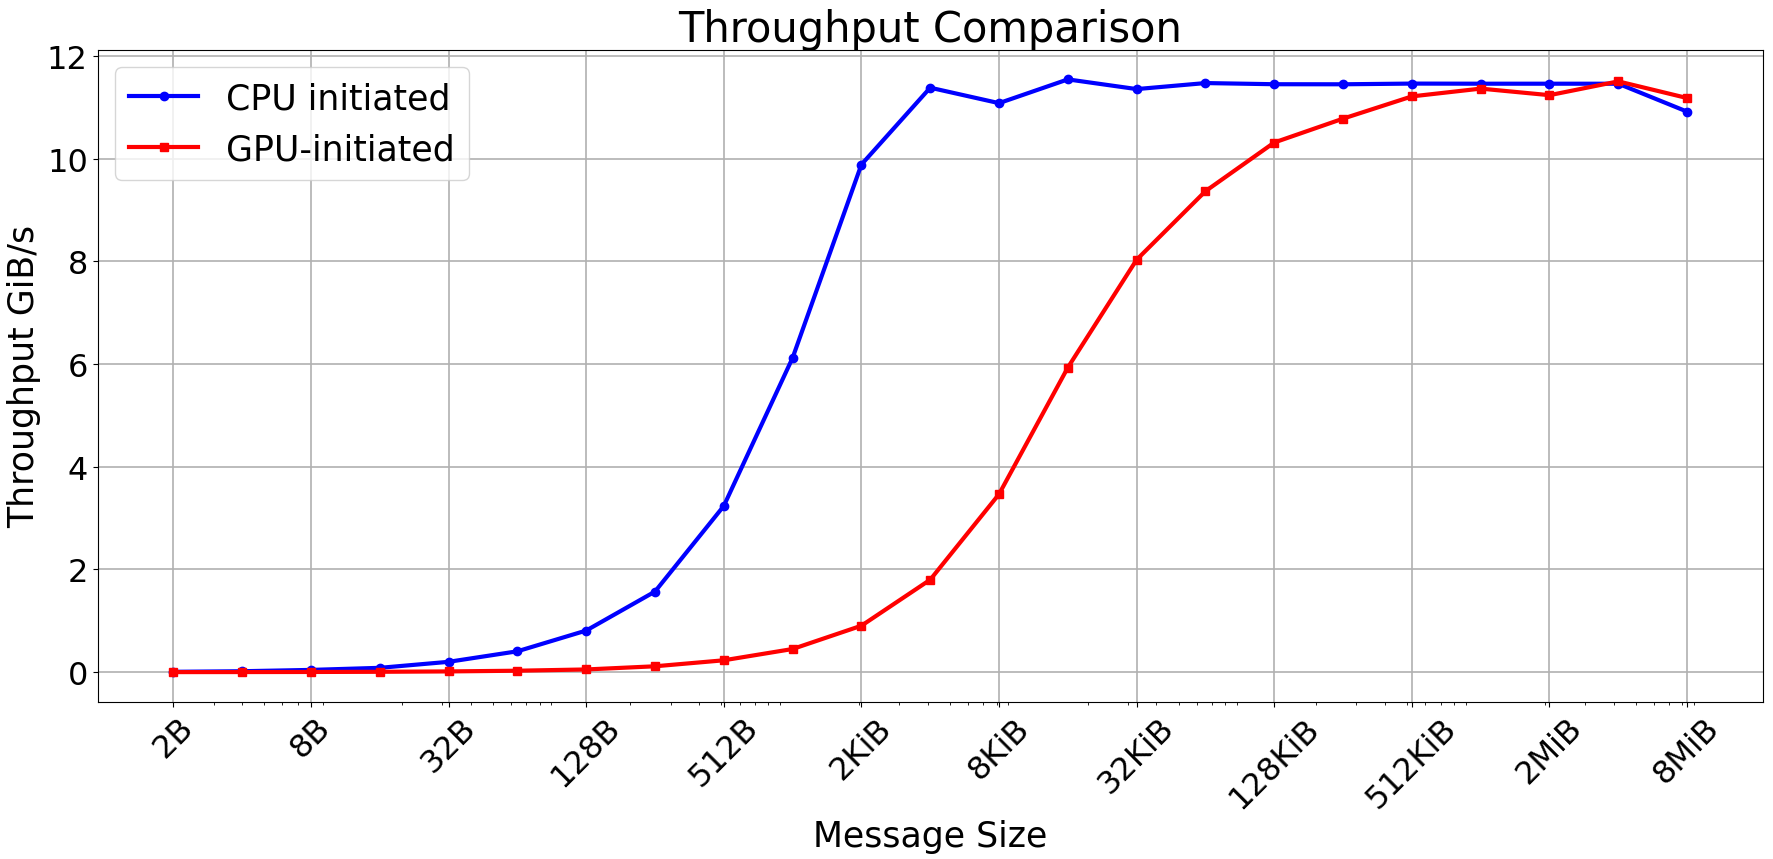
\includegraphics[width=0.7\textwidth]{img/09_gpu_cpu_st.png}
    \caption{Comparison of single-threaded CPU- and GPU-initiated networking performance based on the message size per send call}
    \label{fig:cpu_gpu_st}
\end{figure}

The first benchmark we conducted is visualized in Figure \ref{fig:cpu_gpu_st} and compares the throughput of CPU-initiated RDMA with GPUDirect (blue line) to GPU-initiated communication with NVSHMEM (red line).
In both scenarios, a single CPU thread (or GPU thread respectively) initiates a number of consectutive asynchronous RDMA operations with a certain message size per invocation.
Each invocation incurs some control flow overhead i.e. the instructions needed for asynchronously sending data, and metadata overhead i.e. the header of the messages sent to the NIC and over the network.
With smaller message sizes, the ratio between overhead and payload is greater.
Specifically the control flow overhead limits the throughput if it takes longer to initiate the asynchronous sending from the computing device than it takes from that point on to send the data to the destination.
Consequently, Figure \ref{fig:cpu_gpu_st} shows that larger message sizes increase the system's throughput up to the point where it is limited by the capacity of the physical link (12.5 GB/s).
Comparing the two curves, however, we can see that GPU-initiated communication requires larger message sizes per interface invocation to saturate the physical link limit.
We interpret this as a cause of the higher clock frequency, more powerful instruction set and difference in implementation of the CPU-initiated communication in comparison to the GPU-initiated run.
Thus, an efficient implementation of GPU-initiated shuffle would need to either use larger messages for sending or benefit from some other optimization to compete with a CPU-initiated reference implementation.
One of those optimizations could be a possible parallelization of the send calls across multiple GPU threads.

\begin{figure}[h]
    \centering
    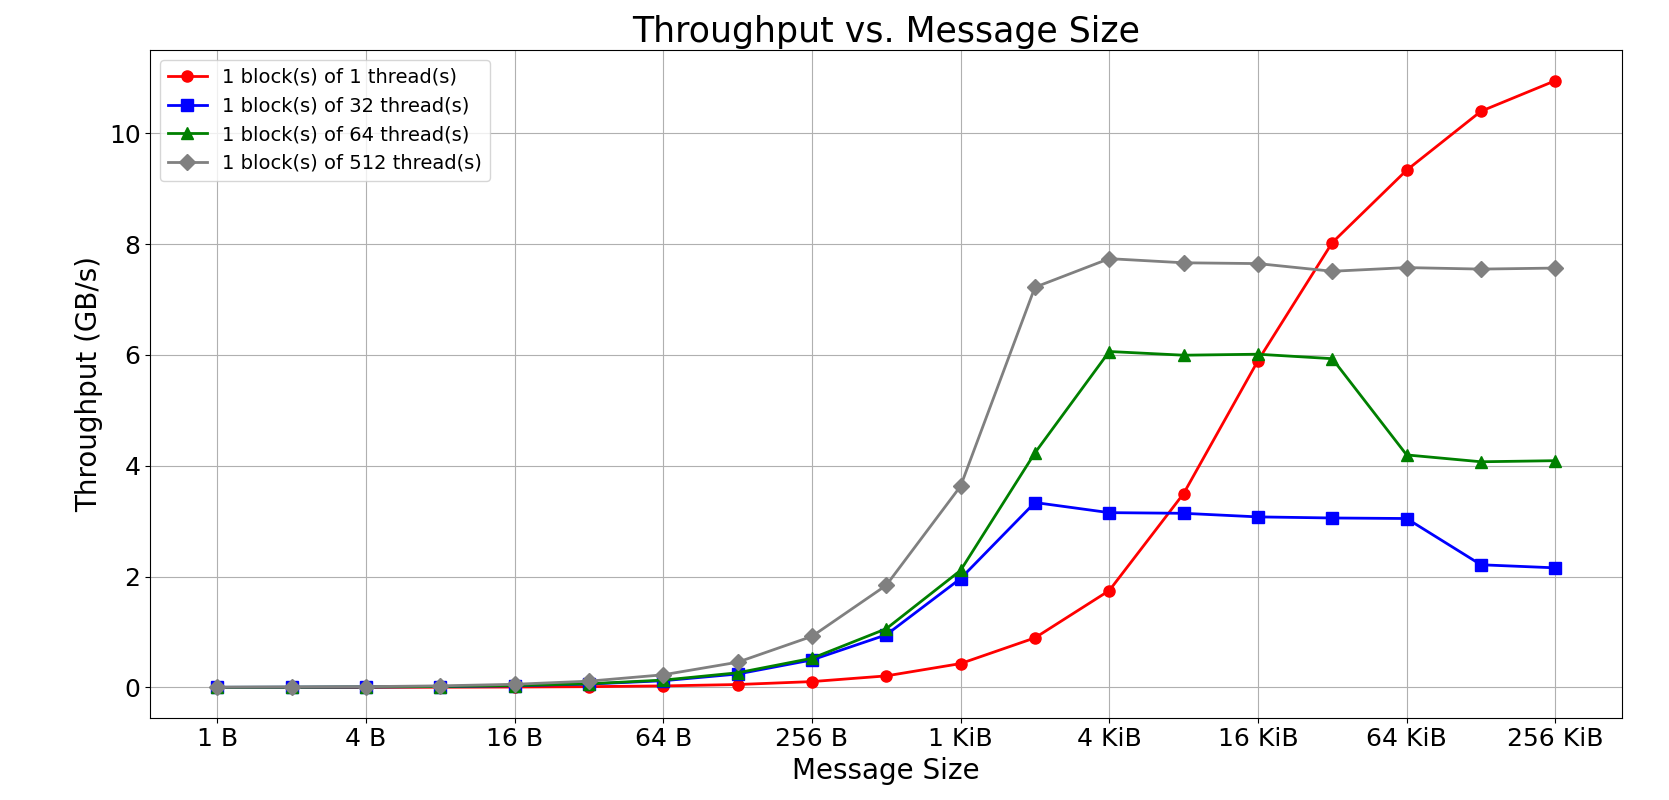
\includegraphics[width=0.8\textwidth]{img/put_granularity_grid1.png}
    \caption{Throughput for repeated nvshmem\_put\_nbi calls using one thread block}
    \label{fig:put_gran_grid_1}
\end{figure}

To analyze the parallelization of send operations in NVSHMEM, we have conducted another series of benchmark which is shown in Figure \ref{fig:put_gran_grid_1}.
These benchmarks use one GPU thread block with a different number of threads and send the messages of the respective size shown on the x-axis using the NVSHMEM asynchronous interface.
Since the read line uses one thread block with one thread, it is equivalent to the red line in the previous plot in Figure \ref{fig:cpu_gpu_st}.
The other lines, which show the results of multiple threads in one block sending the data, show very interesting results.
All of those configurations allow for a faster growth in throughput compared to the single-threaded benchmark depending on the message size.
According to the tested configurations, larger number of threads show this effect more clearly.
Approximately at 4KiB, however, all of the multi-threaded configurations seem to hit some kind of limiting performance factor.
We have not managed to find out the definite reason for this behaviour but are guessing it might be related to the maximum transmission unit (MTU) or a translation look-aside buffer (TLB) related issue.
Without having certainty about the reason for this behaviour, we can nevertheless conclude that using parallelization for sending across threads within a GPU block is not going to be a promising way for the shuffle to work efficiently.

\begin{figure}[h]
    \centering
    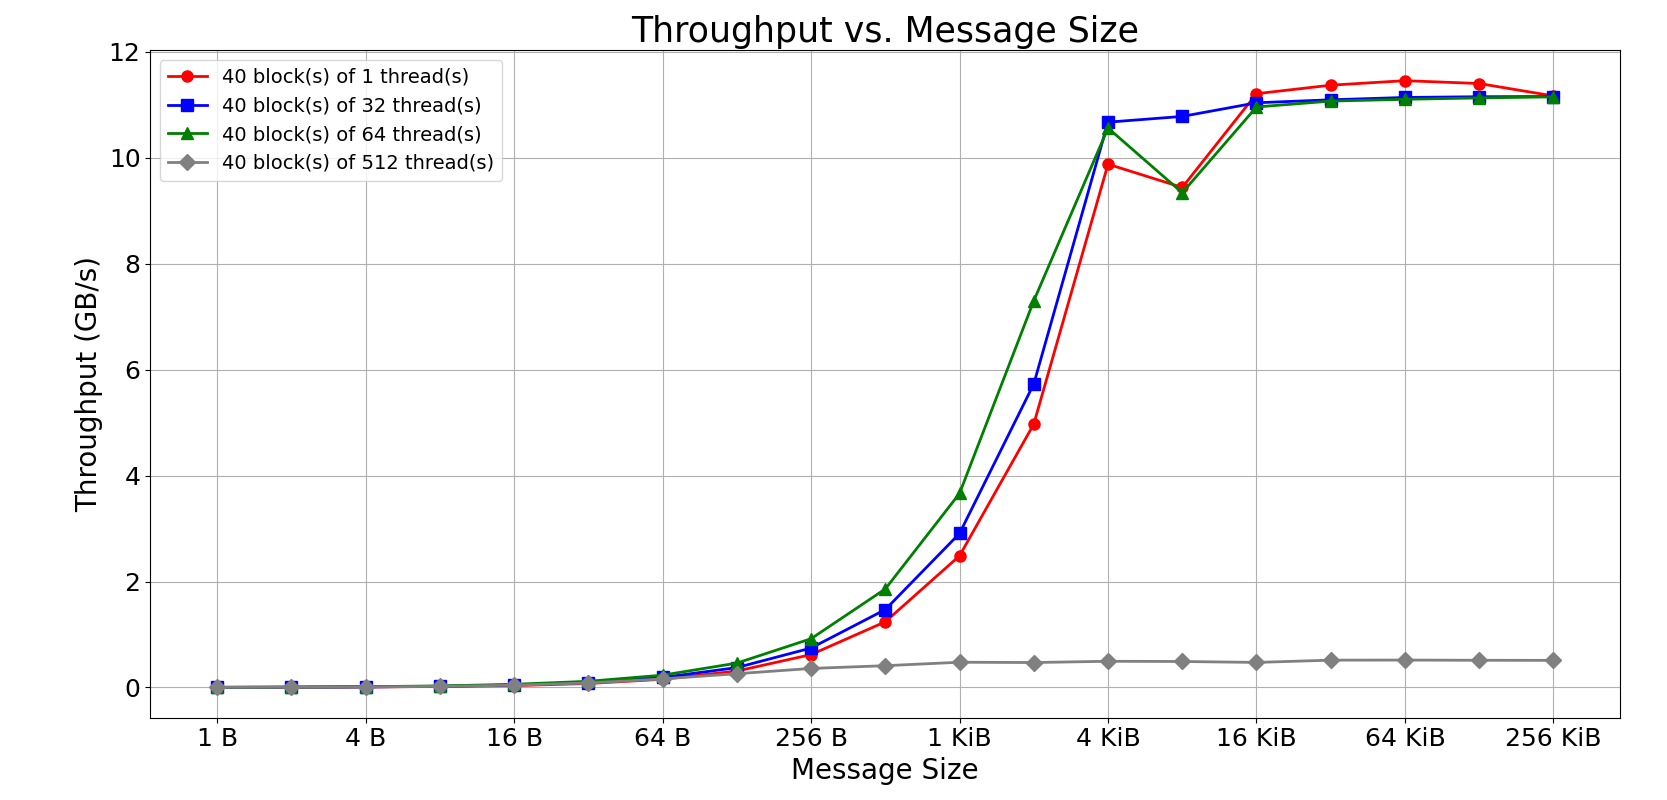
\includegraphics[width=0.8\textwidth]{img/put_granularity_grid40.png}
    \caption{Throughput for repeated nvshmem\_put\_nbi calls using 40 thread blocks}
    \label{fig:put_gran_grid_40}
\end{figure}

To explore other parallelization opportunities, we have run the benchmark again with a different configuration.
This time we are using 40 GPU blocks where each of the blocks includes a certain number of threads as shown in the legend of the plot.
Every of the $n_{threads} \cdot n_{blocks}$ threads in the system again sends messages using the NVSHMEM non-blocking interface.
Surprisingly, this plot shows very different results than the previous one.
Seemingly, the NVSHMEM implementation is not suitable for handling a number of threads as large as 20480 ($40$ blocks $\cdot$ $512$ threads), since the performance is extremely poor, as indicated by the grey line in Figure \ref{fig:put_gran_grid_40}.
On the other hand, all other configurations show very good results, that are comparable to those of CPU-initiated networking shown earlier in Figure \ref{fig:cpu_gpu_st}.
All configurations seem to stagnate just below the physical link bandwidth, which is a sign of good performance.
Nevertheless, we still see some slight performance decrease at around 8 KiB message size for the configurations with one and 64 threads per block, similar to those in the previous plot.
Since the source code of the NVSHMEM library is not publicly available, it is hard to reason further about these results.
But still, this information is very valuable to us for implementing an efficient distributed shuffle using NVSHMEM.
According to the benchmarking results, it should be best to use a large number of blocks (i.e. 40 as used in Figure \ref{fig:put_gran_grid_40}) with a relatively small number of thread per block for sending.
The size of the buffers that are send out should be at least 4KiB to guarantee good sending performance  using the NVSHMEM library.


\section{Implementation}\label{sec:impl}
In this chapter, we describe the implementation of our shuffle algorithm.
We have implemented various versions of the shuffle algorithm, which can be switched using template parameters. As described in Chapter \ref{sec:shufflealgos}, we utilize multi-threaded scanning with one-sided communication. The send buffers can be activated, but the shuffle can also be executed without them. If send buffers are disabled, each tuple is sent directly. If send buffers are activated, one can choose between options (1) atomic insertion and (3) sync-free insertion from Chapter \ref{sec:shuffle:send-buffers}. In all cases of activated send buffers, double buffering is enabled, as described in Chapter \ref{sec:shuffle:double-buffering}. The send buffers are block-local buffers, meaning each block in a grid has its own send buffers that only that block accesses and sends from. 

As seen in the microbenchmark in Chapter \ref{sec:microbench}, it is evident that even with 40 blocks, the message size must be at least 4 KiB to approach the maximum throughput. Therefore, we decided not to assign a fixed size to the send buffer. This allows the send buffer size to be adjusted based on the use case and the number of blocks. It is also observed that sending large buffers from a few block threads outperforms the implementation with small message sizes from many threads. Thus, our implementations with send buffers should significantly outperform those without send buffers, as long as the tuples do not become excessively large. To validate this hypothesis, we have implemented both variants for later testing. We have opted for block-level send buffers because they align with the results of the microbenchmarks, where many blocks with few threads were used. Block-level atomics are more cost-effective than crossing block boundaries, and there is no straightforward method to synchronize threads across block boundaries.

Our shuffle algorithm utilizes a custom implementation of the NVSHMEM \textit{fcollect} primitive to exchange local histograms since it was found that at least \textit{nvshmem\_uint32\_fcollect} does not function when our configuration is compiled in release mode. Furthermore, we use \textit{nvshmem\_putmem\_nbi} to transmit tuples either directly or within the send buffers to the destination PE and \textit{nvshmem\_quiet} to wait for the previous non-blocking call. As mentioned in the preceding paragraph, this currently does not work because the non-blocking interface currently blocks. We also employ \textit{nvshmem\_barrier} to synchronize all PEs, as well as \textit{nvshmem\_malloc} and \textit{nvshmem\_free} to allocate and deallocate symmetric memory.

The runtime of the construction of local histograms scales linearly with the number of tuples since each tuple must be processed once to increase a counter for the destination PE. When the sync-free mode is enabled, an additional $ n_{batches} * n_{pes} * n_{threads\_per\_block} $ iterations are required in each block to create the thread-level histograms. The exchange of our local histograms scales linearly with the number of PEs, and the construction of global histograms is quadratic in the number of PEs.

The tuple scan of the shuffle and insertion into the send buffers runtime scale linearly with the number of tuples. The sending process of the send buffers within the shuffle itself scales linearly with the number of PEs.

In addition to runtime complexity, memory complexity should not be overlooked. For the local histograms, it scales linearly with the number of PEs, and for the global histogram, it is quadratic in the number of PEs. For the thread-level histograms in the sync-free inserts, $ n_{blocks} * n_{threads\_per\_block} * n_{batches} * n_{pes} $ \textit{uint16\_t} (= 2 bytes) are required. Both the local and global histograms' memory is symmetric to allow access via NVSHMEM primitives, whereas local device memory suffices for the thread-level histograms.

The shuffle itself, in addition to the indices of the currently selected buffers for double buffering per block (linear with block count), requires two buffers per block to store the current offsets for each send buffer. This offset buffer encompasses $ 2 * n_{blocks} * n_{pes} $ numbers of type \textit{uint32\_t} (= 4 bytes). Furthermore, a buffer is needed to store the current remote offset per destination, which scales linearly with the number of PEs. Lastly, the send buffers are needed, and due to double buffering, they are required in duplicate. Therefore, the send buffers must accommodate a total of $ 2 * n_{blocks} * n_{threads\_per\_block} * n_{pes} * n_{multiplier} $ tuples. The multiplier can be varied in our shuffle and specifies how many tuples per thread can fit in the send buffer at most.

The mode without a send buffer has the lowest memory complexity but is expected to be slower due to the sending behavior identified in the microbenchmarks in Chapter \ref{sec:microbench}. Sending with a send buffer and atomic increment has lower memory complexity but may have a higher runtime than the sync-free version. It needs to be tested whether the atomic operations cause congestion, potentially offsetting the higher runtime complexity when building the histograms of the sync-free variant.

In our implementation, we assume that each batch contains an equal number of tuples. Consequently, the send buffers provide enough space to hold all tuples in a batch, even if all tuples are sent to the same destination PE. In the reverse scenario, where tuples are evenly distributed, each send buffer is only filled to $ 1 / n_{pes} $, eliminating the need to check whether the buffers are full after each iteration, thereby saving instructions. Double buffering is used to overlap this latency.

The interface of our shuffle algorithm is shown in Listing \ref{lst:shuffle_signature}. It must be called by every PE and offers variations through the parameters as well as compile-time modes, which can be selected via template parameters, along with the tuple type. The passed tuple pointer must be a device pointer.

Within this function, the shuffle is executed in the following sequence:
\begin{enumerate}
    \item  Allocation of histogram buffers.
    \item Scanning of tuples and construction of local histograms.
    \item Exchange of local histograms and construction of global histograms.
    \item Allocation of the send buffer and symmetric memory to receive all tuples.
    \item Scanning of tuples and sending them to the respective destination PE.
    \item Synchronization of all PEs to guarantee the completion of all sending operations.
\end{enumerate}

\begin{lstlisting}[float=htbp, language=C++,caption={Interface of our suffle algorithm},label=lst:shuffle_signature]
template <OffsetMode offset_mode,
            SendBufferMode send_buffer_mode,
            typename Tuple>
__host__ ShuffleResult<Tuple> shuffle(
        uint16_t grid_dimension, uint16_t block_dimension,
        uint8_t send_buffer_size_multiplier,
        const Tuple *device_tuples, uint64_t tuple_count,
        cudaStream_t const &stream, nvshmem_team_t team
)
\end{lstlisting}


\section{Evaluation}\label{sec:eval}
We test the implemented shuffle algorithm by measuring the throughput for varying dimensions of the CUDA grid and thread blocks. As a test setup we use two compute nodes connected by a 100Gb/s Infiniband interconnect. On each node one PE is executed using a NVIDIA V100 GPU. Our setup tests the performance of the shuffle for intra-node communication. Configurations that use both scale-up interconnects on the nodes and scale-out interconnects between the nodes introduce additional behavioural complexity that make it harder to evaluate the effects that are caused by NVSHMEM itself \cite{li2020}. Figure \ref{fig:shuffle_throughput} depicts the result of the shuffle benchmark.

\begin{figure}[h]
    \centering
    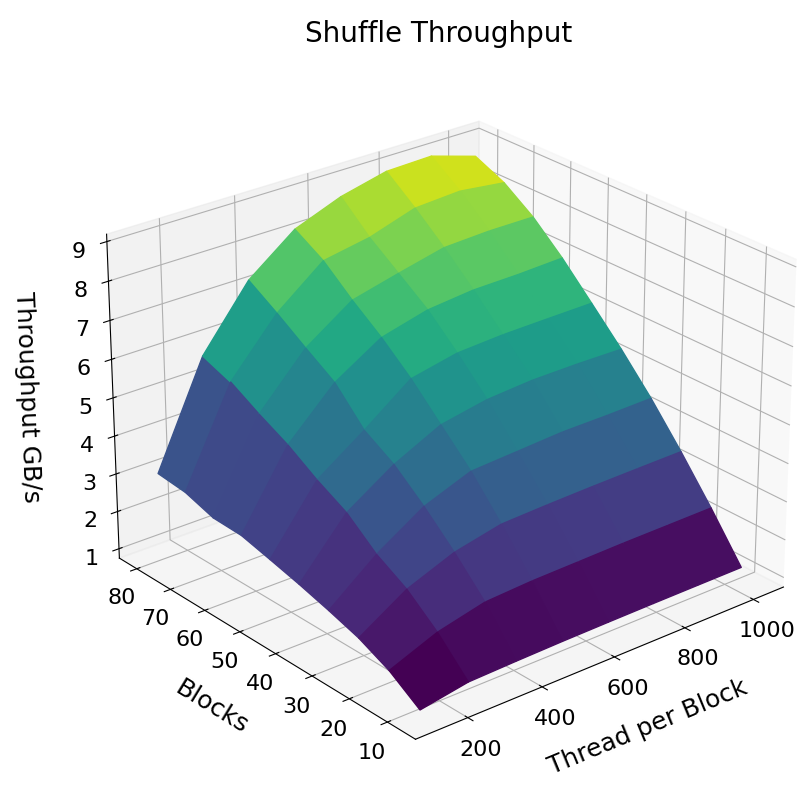
\includegraphics[width=0.6\textwidth]{img/shuffle_throughput.png}
    \caption{Throughput of shuffle algorithm for varying grid and block sizes}
    \label{fig:shuffle_throughput}
\end{figure}

The maximum throughput that can be reached using a high number of sending blocks is just under 9GB/s which would correspond to approximately 70\% of the link bandwidth. Recent work on parallelized CPU-driven shuffling operators using RDMA on the other hand has reported maximum throughput of slightly over 10GB/s \cite{liu2019}. To investigate the limiting factor of the shuffle we test the scanning and inserting of the tuples into the respective send buffers in isolation. Figure \ref{fig:atomic_insert} shows the result for this benchmark using the atomic increment insertion approach.  Notably the results are consistently higher than the link bandwidth. This suggests that the buffer sending introduces an overhead that leads to decreased performance. One aspect that influences the impact of sending on the performance is the correct behaviour of the asynchronous sending operations and intermediate synchronization to ensure buffers are ready for reuse before switching. To this end we conduct a test comparing the blocking send interface of NVSHMEM with the non-blocking asynchronous send interface with different synchronization strategies. As can be seen in Figure \ref{fig:block_nonblock} the execution time differences between the different approaches are negligible. This implies that actually the non-blocking operations do also block. We were not able to find an explanation for this divergence from the specified behaviour and can not make a conclusive statement on whether this is caused by our particular setup or a general problem of the library implementation. With the current implementation our shuffle implementation would directly benefit from correct non-blocking behaviour of the send interface. Based on this we can therefore hypothesize that correcting this error would likely improve our throughput performance.

\begin{figure}
    \centering
    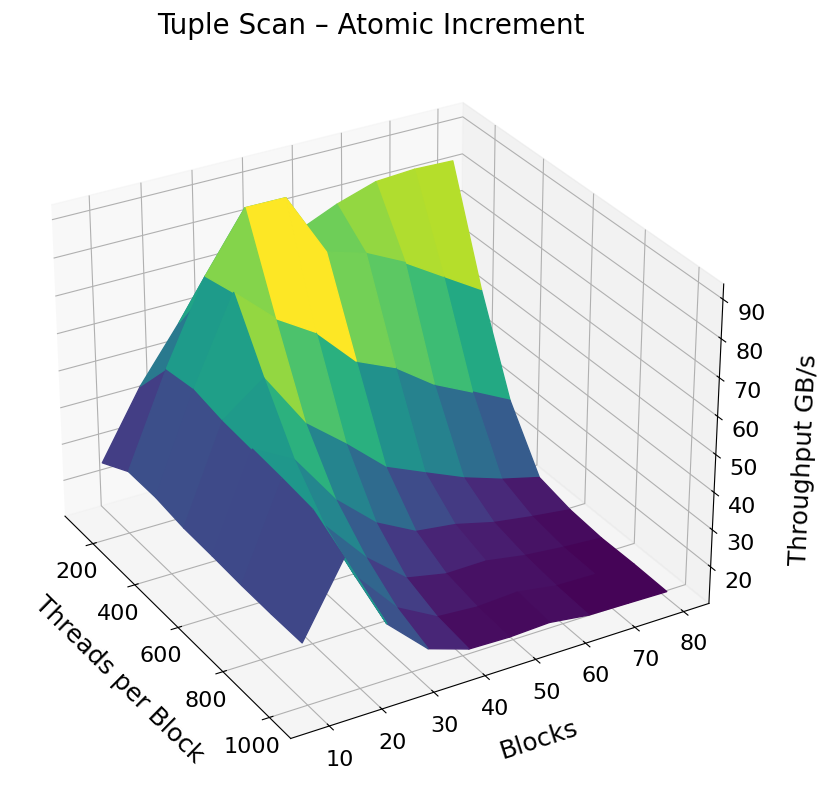
\includegraphics[width=0.6\textwidth]{img/scan_speed_atomic.png}
    \caption{Throughput of tuple scan and insertion using atomic increment as synchronization for varying numbers of blocks and threads}
    \label{fig:atomic_insert}
\end{figure}

\begin{figure}
    \centering
    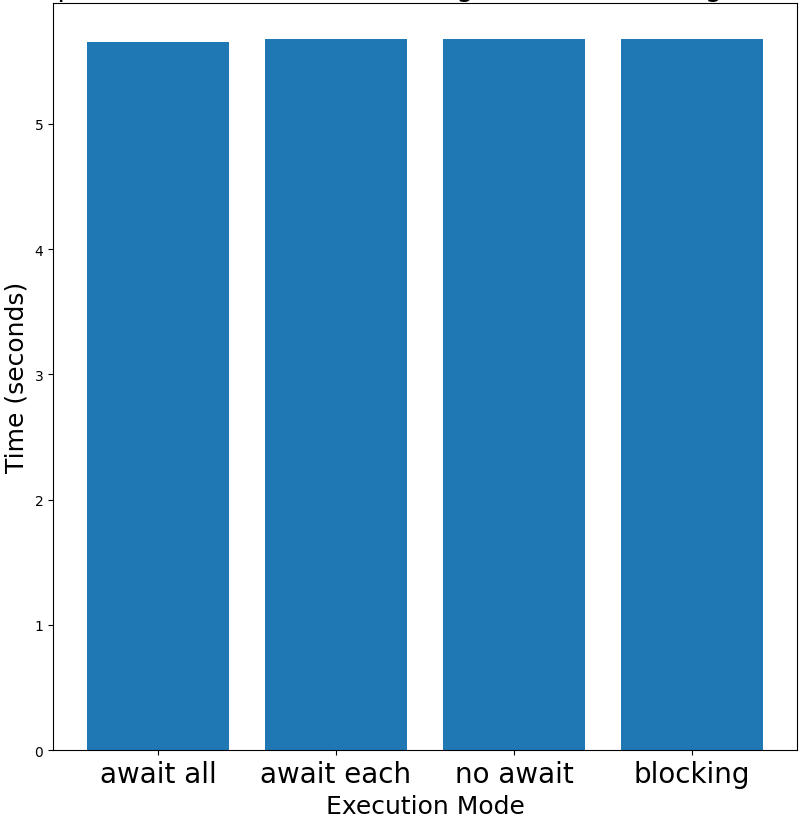
\includegraphics[width=0.4\textwidth]{img/blocking_nonblocking_barchart.png}
    \caption{Different approaches to non-blocking as well as blocking put operations showing the same behaviour}
    \label{fig:block_nonblock}
\end{figure}


\section{Discussion}\label{sec:discuss}
Regarding the question of suitability of NVSHMEM for database usage in general and shuffling in particular we take away the following observations from this work. 
Firstly the performance overhead and behaviour of NVSHMEM-provided communication functions is non trivial to understand. Not only the big configuration space introduced by the two dimensions grid and block size have an impact on the results, but NVIDIA itself states that the underlying interconnect technology can have significant impact on the performance and resulting best practices \cite{NVIDIA2022}. This work is focused on evaluating the case of Infinband communication between nodes and the results apply for this scenario. If additionally other interconnects like NVLINK are used, different approaches might yield better results.
Secondly it has been shown that for the tested configuration the behaviour of the non-blocking interface does not match the specification. The source of this divergence is unclear however this unintended blocking impacts the performance limit of our asynchronous communication approach. Further investigation is needed to determine the concrete cause and possibly correct configuration errors.
Further the NVSHMEM programming model and memory model is primarily intended for use in high performance computing scenarios. The symmetric memory abstraction requires preallocating memory before launching a kernel and dynamic memory management during kernel run time is severely limited. Also the launcher based library initialization is not natural for usage in DBMS where operators are dynamically launched for different queries and table sizes and memory requirements can therefore not be known beforehand. It also impedes elasticity, an important topic in today's cloud database systems. 
Lastly our approach, partly as a consequence of NVSHMEM's limitations, assumes that all tuples for shuffling fit in memory of the GPU (16GB in the tested scenario). This requirement can not be imposed in general cases and is in fact unlikely to hold in practical scenarios considering the sizes database tables can reach. Further work towards more complex dynamic batched shuffling is needed to mitigate this limitation.

\section{Conclusion and Outlook}\label{sec:conclusion}
This paper explored the potential of NVSHMEM for enhancing the performance of communication-intensive workloads such as shuffling operations in distributed database systems.
Using NVSHMEM, we were able to leverage GPU-initated communication - as opposed to the traditional CPU-initiated approach - for optimized data transfers.

We made several key findings and contributions in this paper.
Using NVSHMEM, we built a GPU-initiated shuffle algorithm and benchmarked it, evaluating multiple algorithmic options.

Our microbenchmarks demonstrate that while NVSHMEM can achieve reasonable throughput, it also exhibits performance characteristics that are non-trivial to understand and do not align with initial expectations.

Additionally, we found out that while the use of NVSHMEM can reduce the kernel launch overhead, it comes at the cost of a more complex programming model, requiring careful design for communication between the host and device.

While NVSHMEM shows clear potential for performance improvements, it is not clear whether this approach is appropriate for general database applications.
In future work, a deeper dive into the intricacies of NVSHMEM's internal workings is warranted to explore its usefulness in a distributed database context.


% Points to mentions: investigated performance aspects of nvshmem by means of microbenchmarks. Implemented a shuffling algorithm with different approaches for sending and synchronization. Nvshmem was not designed for use in a database environment which makes adaption complicated.

\printbibliography

\end{document}